\chapter{Architecture visualization: C4 notation}

\section{Visualizing software architecture}
There are not only one diagrams to visualize software architecture,
but many of them.

Variety of goals, stakeholders, focus, etc.


\section{Issues in sw architecture visualization}

\begin{itemize}
  \item Purpose of elements (boxes, arrows, etc.)
  \item Relationship between elements
  \item Levels of abstraction
  \item No context or logical starting point
  \item Consistency between diagrams
  \item Require explanations or descriptions to be fully understood
\end{itemize}

Diagrams are like maps: different providers, google or openstreetmap have different purposes.
For this reason, we will introduce the C4 model, which is a standard for software architecture visualization.



\section{C4 Model}

With this model we can zoom-in and zoom-out to navigate through the different
levels of abstraction to use with different stakeholders.


\begin{flushleft}
  \begin{minipage}{0.67\linewidth}
    \raggedright
    A \textbf{software system} is made up of one or more \textbf{containers}, each of
    which contains one or more \textbf{components}, which in turn are implemented by
    one or more code elements. And \textbf{people} use the software systems that we
    build.\newline

    It is organized in 4 levels of abstraction:
    \begin{itemize}
      \item Software System
      \item Container
      \item Component
      \item Code Element
    \end{itemize}
  \end{minipage}%
  \hfill
  \begin{minipage}{0.27\linewidth}
    \centering
    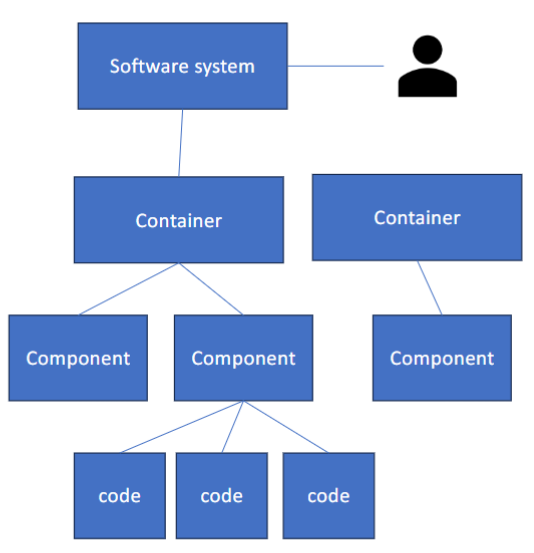
\includegraphics[width=\linewidth]{images/Architecture-visualization/AV-esempio1.png}
    \captionof{figure}{Static structure}
  \end{minipage}
\end{flushleft}

\subsection{Container}
A boundary inside which some code is executed or some data is stored.
Containers are \textbf{separately deployable}.

\paragraph{Examples: }
\begin{itemize}
  \item Application (server-side or client side)
  \item Database, file system, etc.
  \item Microservice (if not a system per se)
  \item Mobile app
  \item Script (python, shell, R, etc.)
\end{itemize}


\subsection{Component}

A grouping of related functionality encapsulated behind a well-defined interface

Components are \textbf{NOT} separately deployable and how
components are packaged is not relevant at this level.

\subsection{Code}

The basic building blocks of a programming language:
\begin{itemize}
  \item classes,
  \item interfaces,
  \item functions,
  \item objects,
  \item enums
\end{itemize}


\section{Different type of diagrams}

The C4 model defines different types of diagrams for each level of abstraction.

\begin{itemize}
  \item \textbf{Context diagram}: it shows how the software system in scope fits into
        the context around it.
  \item \textbf{Container diagram}: it shows the high-level technical building blocks
        (containers) and how they interact.
  \item \textbf{Component diagram}: it shows the components inside each container
  \item \textbf{Code diagram}: it shows how a component is implemented
\end{itemize}


\begin{figure}[h!]
  \centering
  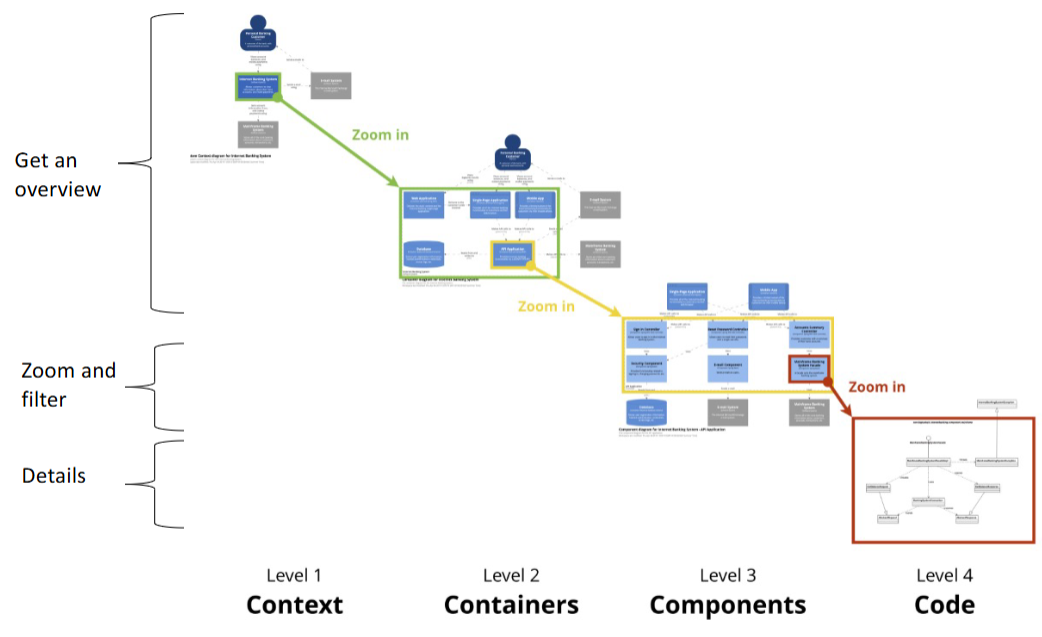
\includegraphics[width=0.5\linewidth]{images/Architecture-visualization/AV-esempio2.png}
\end{figure}

Using the SPG, Solidarity Purchasing Group, presented before, as an example, we can create different diagrams for each level of abstraction.


\section{Level 1: Context diagram}

It helps answering such questions:

\begin{itemize}
  \item What is the software system that we are building (or have built)?
  \item Who is using it?
  \item How does it fit in with the existing environment?
\end{itemize}

It is \textbf{required}: it is the starting point for communicating with any stakeholder

The key elements of a context diagram are:

\begin{itemize}
  \item People who will use the software system
  \item Other software systems with which the reference system interacts
  \item + optionally the organization boundary
\end{itemize}
Interaction between elements: Directed arrows with high-level information about
the purpose of that interaction.
We can connect elements with arrows. It is
better to use only one way arrows and not to use bidirectional once.



\begin{flushleft}
  \begin{minipage}{0.65\linewidth}
    \raggedright
    \subsection{Information reported - People}

    The people element have:

    \begin{itemize}
      \item \textbf{Name}: the name of the person, user, role, actor or persona.
      \item \textbf{Description}: A short description of the person, their role,
            responsibilities, etc
    \end{itemize}

  \end{minipage}%
  \hfill
  \begin{minipage}{0.3\linewidth}
    \centering
    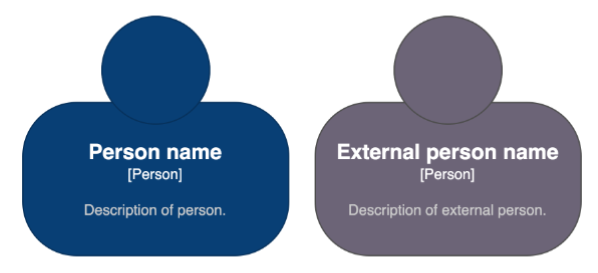
\includegraphics[width=\linewidth]{content/chapters/images/2026-03-22-11-53-33.png}
  \end{minipage}
\end{flushleft}


\begin{flushleft}
  \begin{minipage}{0.65\linewidth}
    \raggedright
    \subsection{Information reported - Software system}

    The software system element have:

    \begin{itemize}
      \item \textbf{Name}: The name of the software system.
      \item \textbf{Description}: A short description of the software system, its goal
            and responsibilities, etc.
    \end{itemize}
  \end{minipage}%
  \hfill
  \begin{minipage}{0.3\linewidth}
    \centering
    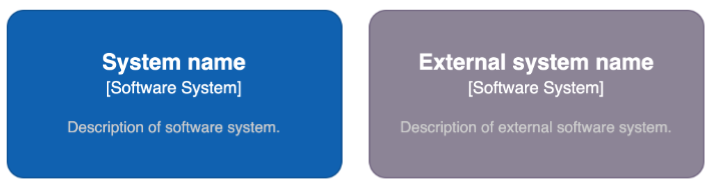
\includegraphics[width=\linewidth]{content/chapters/images/2026-03-22-11-58-07.png}
  \end{minipage}
\end{flushleft}


\begin{figure}[h!]
  \centering
  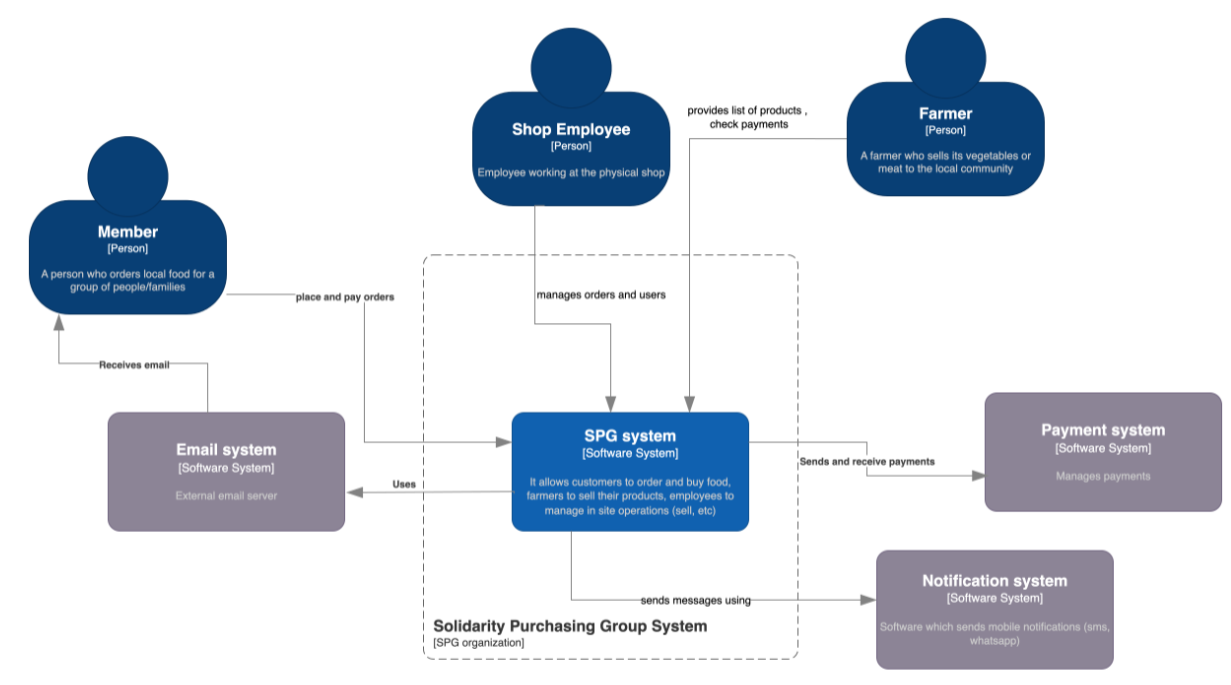
\includegraphics[width=0.5\linewidth]{content/chapters/images/2026-03-22-11-59-04.png}
\end{figure}


\section{Level 2: Container diagram}


Goal: illustrate the high-level technology elements and how responsibilities are
distributed across elements and how containers communicate with each other


Every container must be deployable independently and the diagram is \textbf{required} and readed by
software development adn operations stuff.






\begin{flushleft}
  \begin{minipage}{0.65\linewidth}
    \raggedright
    \subsection{Elements}
    People, software systems and containers. For each container:

    \begin{itemize}
      \item Name: The name of the container (e.g. ``Internet-facing web server'',
            ``Database'', etc).
      \item Technology: The implementation technology (e.g. Java/Spring MVC
            application,
            ASP.NET web application, Relational Database Schema, etc.) or the general type
            of technology''
      \item Description: A short descriptive statement, or perhaps a list of the
            container's key responsibilities or entities/tables/files/etc. that are being stored.
    \end{itemize}

    System boundary must be coherent with L1

  \end{minipage}%
  \hfill
  \begin{minipage}{0.3\linewidth}
    \centering
    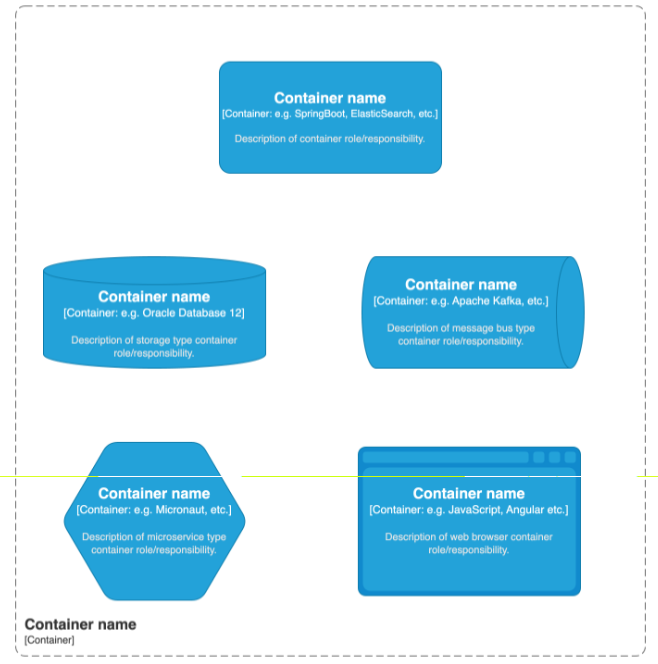
\includegraphics[width=\linewidth]{content/chapters/images/2026-03-22-12-05-11.png}
  \end{minipage}
\end{flushleft}



\begin{flushleft}
  \begin{minipage}{0.65\linewidth}
    \raggedright
    \subsection{Interactions between containers}
    Interactions between containers must be as explicit as possible.


    Example of useful information to annotate the interactions with:

    \begin{itemize}
      \item The purpose of the interaction (e.g. ``reads/writes data from'', ``sends
            reports to'', etc).
      \item The communication mechanism (e.g. REST, Web API, Java Message Service,
            Web Services ).
      \item The communication style (e.g. synchronous, asynchronous, batched,
            twophase commit, etc).
      \item Protocols and port numbers (e.g. HTTP, HTTPS, SOAP/HTTP, SMTP, FTP,
            RMI/IIOP, etc)
    \end{itemize}
  \end{minipage}%
  \hfill
  \begin{minipage}{0.3\linewidth}
    \centering
    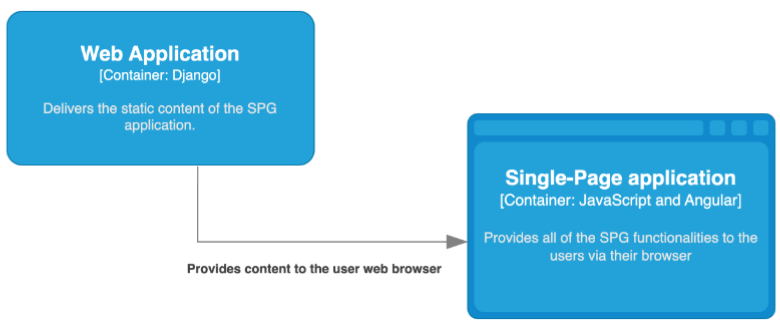
\includegraphics[width=\linewidth]{content/chapters/images/2026-03-22-12-08-20.png}
  \end{minipage}
\end{flushleft}


\begin{figure}[h!]
  \centering
  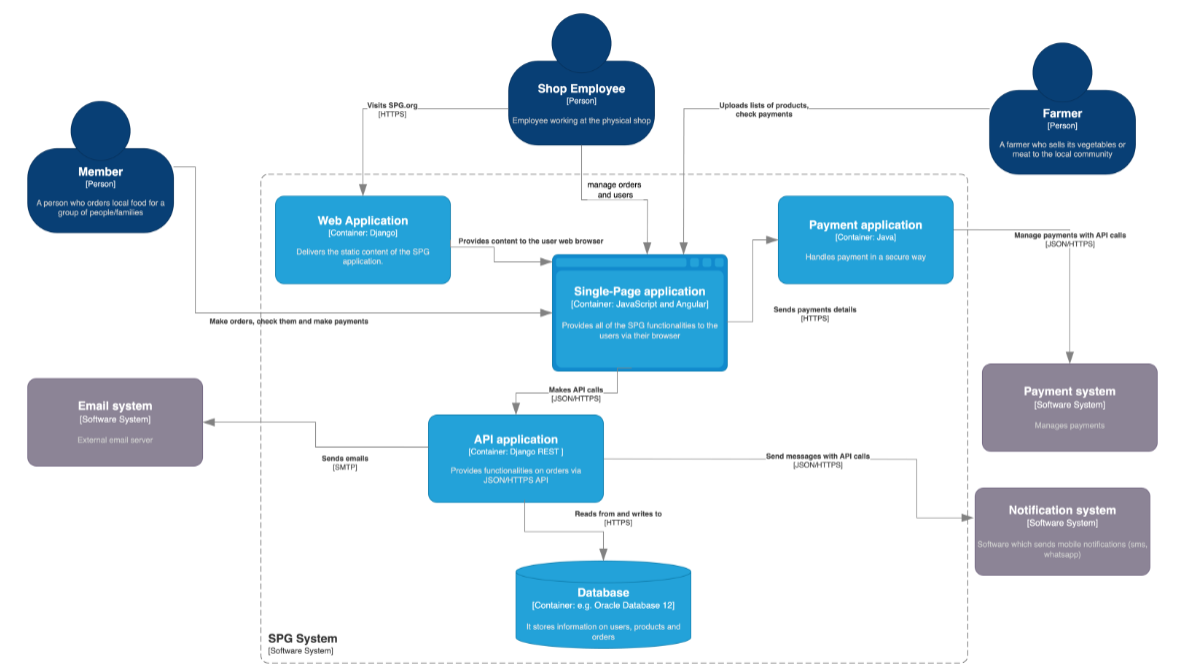
\includegraphics[width=0.6\linewidth]{content/chapters/images/2026-03-22-12-07-46.png}
\end{figure}

\section{Level 3: Components diagram}


It shows components that are within a single container at a time.
Infrastructural elements (e.g. , logging, metering) and shared library might
be annotated, separated, or excluded.

It helps to answer the questions like

\begin{itemize}
  \item What components is each container made up of?
  \item Do all components stay within in a container?
  \item How components interact each other ?
  \item How the software works at a high-level?
\end{itemize}

Optional, especially for containers like data storage, microservices.
It is for technical people within the software development team.



\begin{flushleft}
  \begin{minipage}{0.65\linewidth}
    \raggedright
    \subsection{Elements}
    Same of the containers + components: people, software systems, containers and components.

    Information to show for each component:
    \begin{itemize}
      \item Name: The name of the component.
      \item Technology: The implementation technology for the component (e.g.
            Java, Object, C\#, Ruby).
      \item Description: A short description of the component in terms of its
            responsibilities
    \end{itemize}
  \end{minipage}%
  \hfill
  \begin{minipage}{0.3\linewidth}
    \centering
    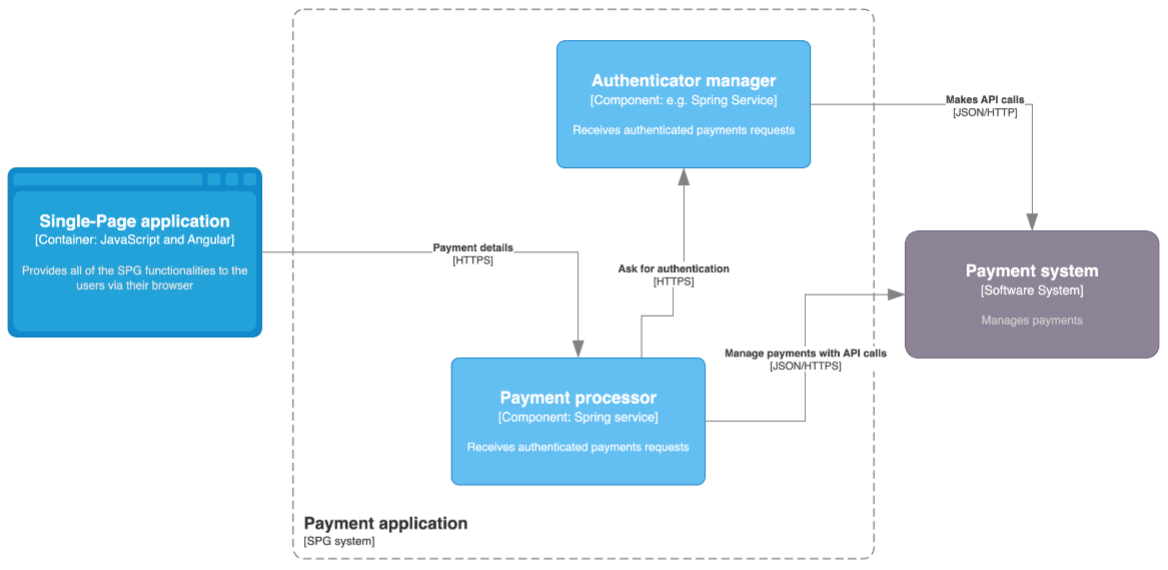
\includegraphics[width=\linewidth]{content/chapters/images/2026-03-22-12-24-09.png}
  \end{minipage}
\end{flushleft}

\begin{figure}[h!]
  \centering
  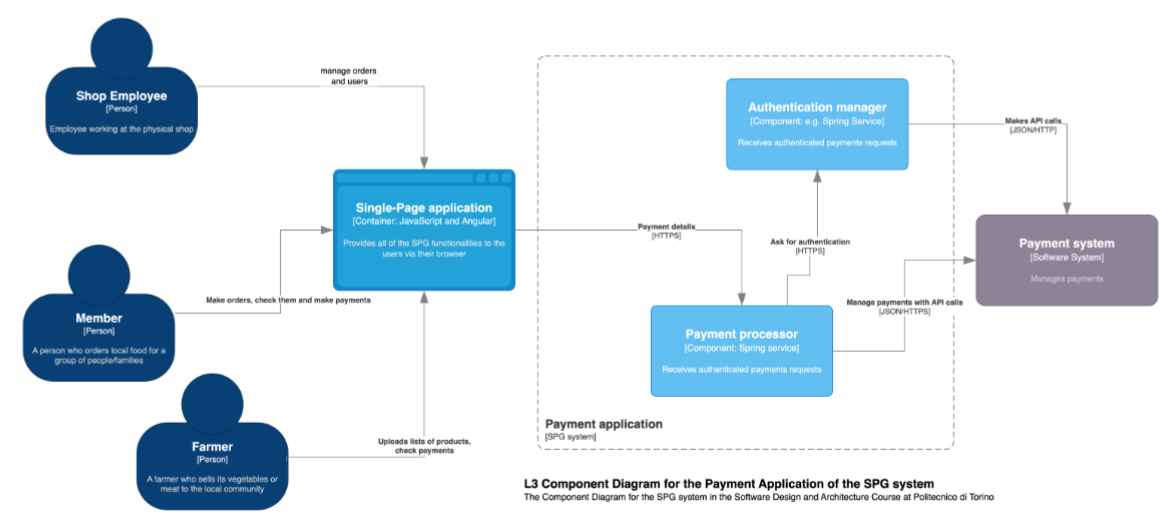
\includegraphics[width=0.65\linewidth]{content/chapters/images/2026-03-22-12-24-41.png}
\end{figure}

The UML component diagram is useful to provide more detailed documentation.


\begin{center}
  \begin{minipage}{0.75\linewidth}
    \begin{minipage}{0.47\linewidth}
      \centering
      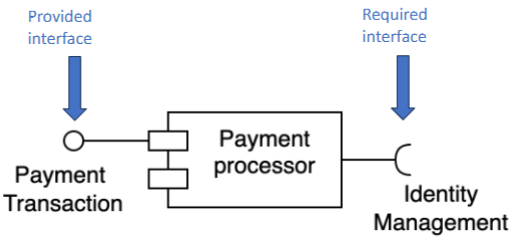
\includegraphics[width=\linewidth]{content/chapters/images/2026-03-22-12-25-47.png}
    \end{minipage}%
    \hfill
    \begin{minipage}{0.47\linewidth}
      \centering
      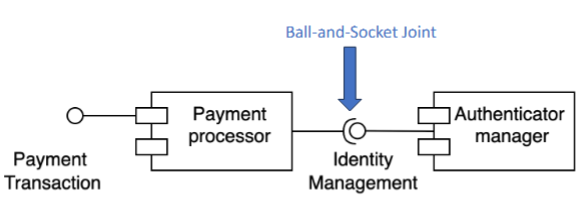
\includegraphics[width=\linewidth]{content/chapters/images/2026-03-22-12-25-56.png}
    \end{minipage}
  \end{minipage}%
\end{center}

\subsubsection{Ports}

Ports indicate that required/provided interfaces are
delegated to an internal class.

\begin{figure}[h!]
  \centering
  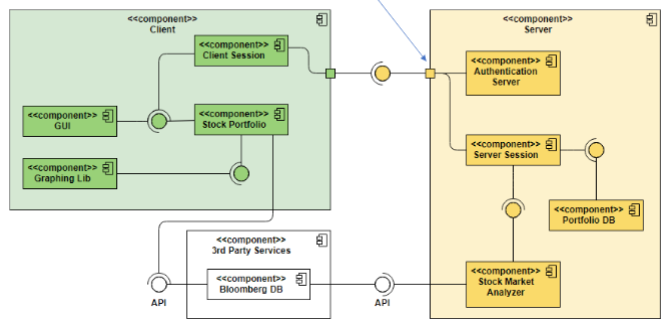
\includegraphics[width=0.65\linewidth]{content/chapters/images/2026-03-22-12-26-49.png}
\end{figure}



\section{Level 4: Code diagram}

\begin{flushleft}
  \begin{minipage}{0.65\linewidth}
    \raggedright
    It shows the implementation details of an individual component, it helps
    bridging the gap between architecture and code.

    Usually, UML class diagrams are used beacuse:
    \begin{itemize}
      \item They can be generated automatically (e.g., with PlantUML)
      \item Large amount of details !
    \end{itemize}

    This is not mandatory, it is optional and it is especially for software
    developers, and more in general for technical people within the software
    development team.

  \end{minipage}%
  \hfill
  \begin{minipage}{0.3\linewidth}
    \centering
    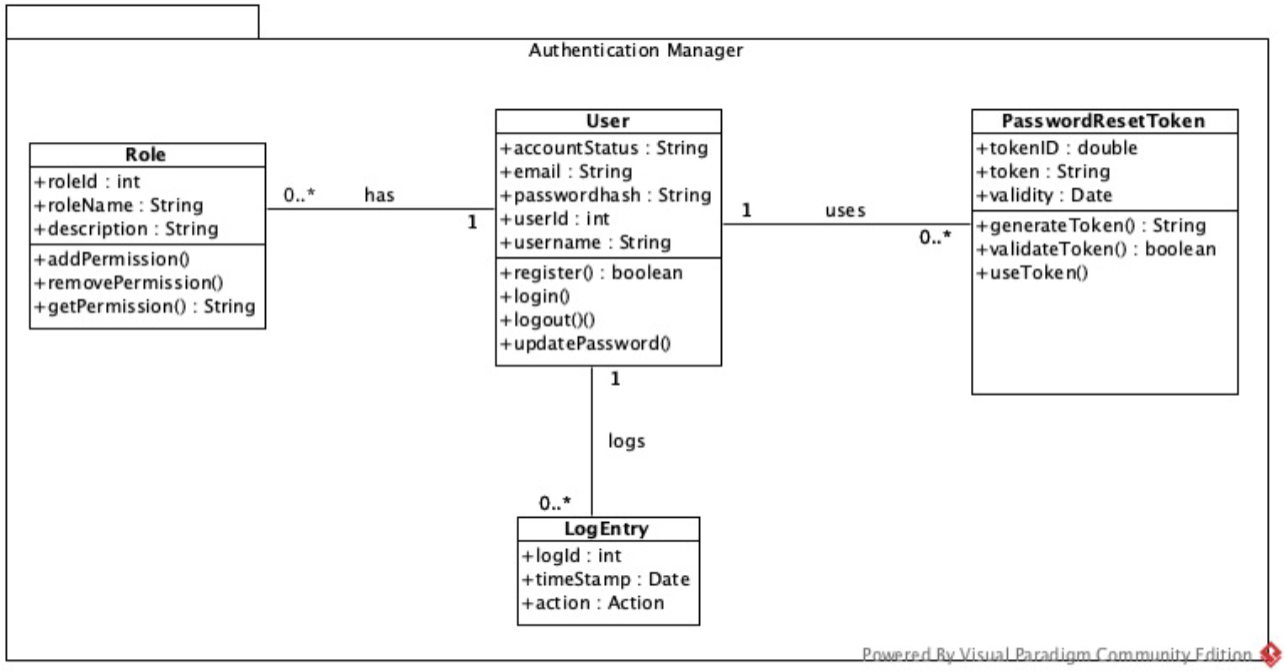
\includegraphics[width=\linewidth]{content/chapters/images/2026-03-22-12-29-18.png}
  \end{minipage}
\end{flushleft}


We can use Draw.io but no check on syntax. Instead we can use
\url{https://academic.signavio.com/p/login}.

Coerence between levels are important for exam.

\section{Summary of C4 model}
A lightweight notation to visualize the static structure of a software system
It is based on a hierarchic conceptual model of software systems. 4 levels (2 of which mandatory).

Four main elements, associated with unidirectional lines, directions shown is the most relevant.

Customizable with colors , shapes, lines
\begin{itemize}
  \item line styles for synchronous/asynchronous communication;
  \item colors for different components;
  \item different shapes for specific types of components;
\end{itemize}






